\section{Schaffer Function N.4}
  The \emph{Schaffer Function N.4}...

  \begin{definition}[Schaffer Function N.4]
    ...
  \end{definition}

    \begin{figure}[ht!]
    \centering
    \begin{subfigure}[b]{0.45\textwidth}
      \centering
      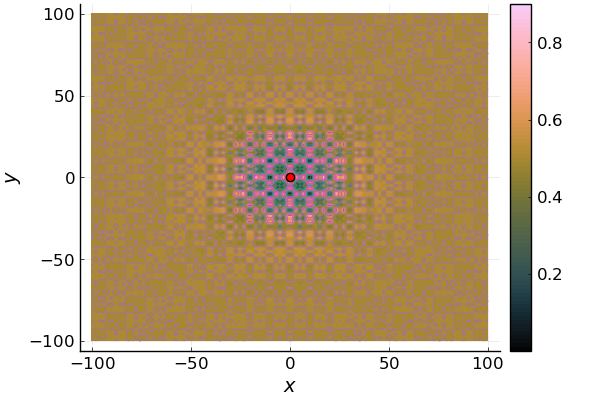
\includegraphics[width=\textwidth]
        {img/test_functions/schaffer_2_contour.png}
      \caption{Contour plot of the Schaffer Function N.2}
    \end{subfigure}
    \hfill
    \begin{subfigure}[b]{0.45\textwidth}
      \centering
      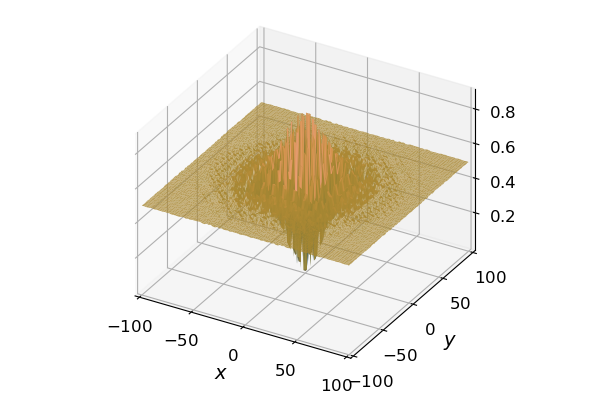
\includegraphics[width=\textwidth]
        {img/test_functions/schaffer_2_surface.png}
      \caption{Surface plot of the Schaffer Function N.2}
    \end{subfigure}
    \caption{
      Visualization of the Schaffer Function N.2.
      The contour and surface plots illustrate the function's topology, with the
      global minimum denoted by a red dot.
    }
    \label{fig:app:test:schaffer_2}
  \end{figure}
